%                      Code_Saturne version 1.3
%                      ------------------------
%
%     This file is part of the Code_Saturne Kernel, element of the
%     Code_Saturne CFD tool.
% 
%     Copyright (C) 1998-2007 EDF S.A., France
%
%     contact: saturne-support@edf.fr
% 
%     The Code_Saturne Kernel is free software; you can redistribute it
%     and/or modify it under the terms of the GNU General Public License
%     as published by the Free Software Foundation; either version 2 of
%     the License, or (at your option) any later version.
% 
%     The Code_Saturne Kernel is distributed in the hope that it will be
%     useful, but WITHOUT ANY WARRANTY; without even the implied warranty
%     of MERCHANTABILITY or FITNESS FOR A PARTICULAR PURPOSE.  See the
%     GNU General Public License for more details.
% 
%     You should have received a copy of the GNU General Public License
%     along with the Code_Saturne Kernel; if not, write to the
%     Free Software Foundation, Inc.,
%     51 Franklin St, Fifth Floor,
%     Boston, MA  02110-1301  USA
%
%-----------------------------------------------------------------------
%

%%%%%%%%%%%%%%%%%%%%%%%%%%%%%%%%%%
%%%%%%%%%%%%%%%%%%%%%%%%%%%%%%%%%%
\section{Discr\'etisation}
%%%%%%%%%%%%%%%%%%%%%%%%%%%%%%%%%%
%%%%%%%%%%%%%%%%%%%%%%%%%%%%%%%%%%

\begin{figure}[h]
\parbox{8cm}{%
\centerline{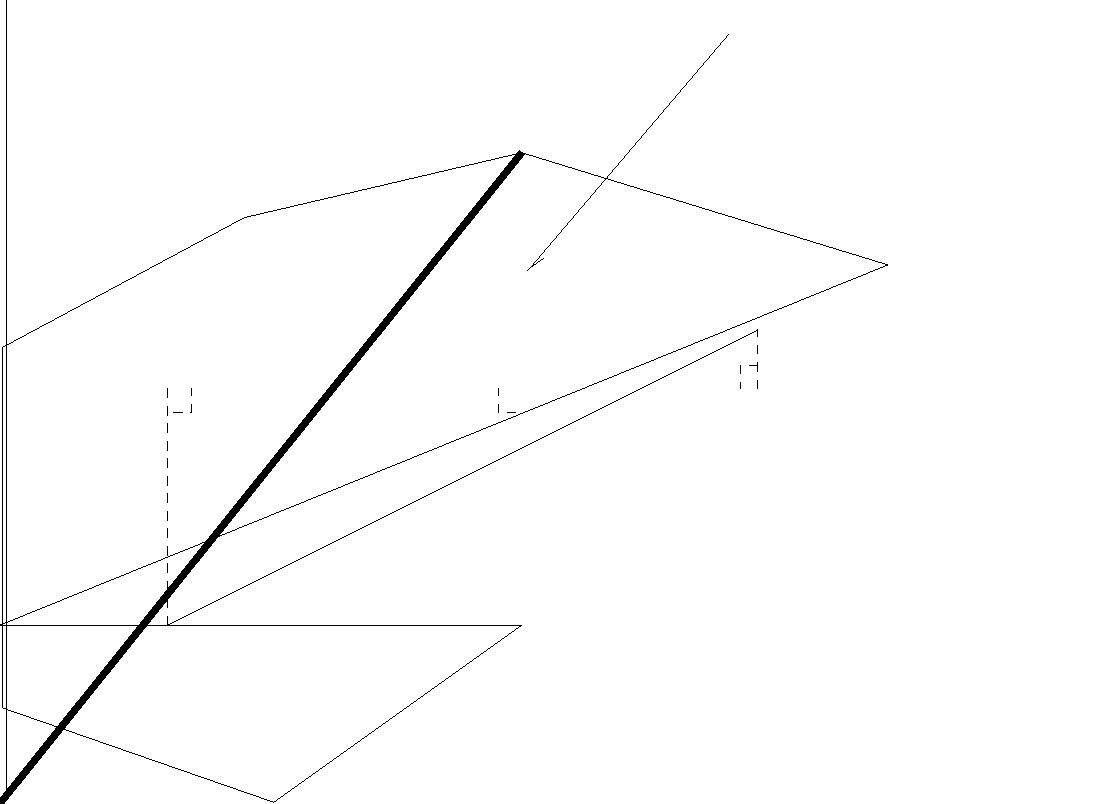
\includegraphics[height=4cm]{../Base/Gradmc/Images/facette.pdf}}}
\parbox{8cm}{%
\centerline{
\includegraphics[height=4cm]{../Base/Gradmc/Images/facebord.pdf}}}
\caption{\label{Base_Gradmc_fig_geom_gradmc}D\'efinition des diff\'erentes entit\'es
g\'eom\'etriques pour les faces internes (gauche) et de bord (droite).}
\end{figure}

On se reportera aux notations de la figure \ref{Base_Gradmc_fig_geom_gradmc}. 
On cherche \`a calculer $\vect{G}_{c,i}$, gradient au centre de la cellule $i$ de la
fonction scalaire $P$. Soit  $\vect{G}_{f,ij}\,.\,\vect{d}_{ij}$ une estimation
\`a la face $ij$ (dont les voisins sont les cellules $i$ et $j$) 
du gradient projet\'e dans la direction du vecteur $\vect{d}_{ij}$ (\`a pr\'eciser). 
De m\^eme, on note 
$\vect{G}_{fb,ik}\,.\,\vect{d}_{b,ik}$ une estimation  \`a la face de bord $ik$
($k^{\text{i\`eme}}$ face de bord appuy\'ee sur la cellule $i$) du gradient projet\'e dans
la direction du vecteur $\vect{d}_{b,ik}$ (\`a pr\'eciser). 
L'id\'eal serait de pouvoir trouver un vecteur $\vect{G}_{c,i}$ tel que, pour toute
face interne $ij$ ($j\in Vois(i)$) et toute face de bord $ik$
($k\in\gamma_b(i))$, on ait~:
\begin{equation}
\left\{\begin{array}{c}
\vect{G}_{c,i}\,.\,\vect{d}_{ij}=\vect{G}_{f,ij}\,.\,\vect{d}_{ij}\\
\vect{G}_{c,i}\,.\,\vect{d}_{b,ik}=\vect{G}_{f,b,ik}\,.\,\vect{d}_{b,ik}
\end{array}\right.
\end{equation}




Comme il est g\'en\'eralement impossible d'obtenir l'\'egalit\'e, on cherche 
\`a minimiser la fonctionnelle~$\mathcal{F}_i$ suivante~:
\begin{equation}\label{Base_Gradmc_eq_fonctionnelle_gradmc}
\mathcal{F}_i(\vect{G}_{c,i},\vect{G}_{c,i})=
\frac{1}{2}\sum\limits_{j\in Vois(i)}\left[
\vect{G}_{c,i}\,.\,\vect{d}_{ij}-\vect{G}_{f,ij}\,.\,\vect{d}_{ij}
\right]^2+
\frac{1}{2}\sum\limits_{k\in \gamma_b(i)}\left[
\vect{G}_{c,i}\,.\,\vect{d}_{b,ik}-\vect{G}_{f,b,ik}\,.\,\vect{d}_{b,ik}
\right]^2
\end{equation}

Pour ce faire, on annule la d\'eriv\'ee de
$\mathcal{F}_i(\vect{G}_{c,i},\vect{G}_{c,i})$ 
par rapport \`a
chacune des trois composantes ($G_{c,i,x}, G_{c,i,y}, G_{c,i,z}$) du vecteur
inconnu $\vect{G}_{c,i}$ et l'on r\'esout le syst\`eme qui en r\'esulte.

Pour pouvoir inverser le syst\`eme localement et donc \`a faible co\^ut, on
cherche \`a \'eviter les d\'ependances de $\vect{G}_{f,ij}\,.\,\vect{d}_{ij}$ et 
de $\vect{G}_{f,b,ik}\,.\,\vect{d}_{b,ik}$ au gradient $\vect{G}_{c,j}$
(gradient pris dans les cellules voisines). Un choix particulier du vecteur
$\vect{d}$ permet d'atteindre ce but~:
\begin{equation}
\vect{d}_{ij} = \frac{\vect{IJ}}{||\vect{IJ}||} \text{\ \ et\ \ } \vect{d}_{b,ik} = \frac{(\vect{I'F})_l}{||\vect{I'F}||}=\vect{n}_{b,ik}
\end{equation}


Ainsi, pour les faces internes, le vecteur $\vect{d}$ est le vecteur norm\'e joignant
le centre des cellules voisines. La quantit\'e
$\vect{G}_{f,ij}\,.\,\vect{d}_{ij}$ est reli\'ee directement aux
valeurs de la variable $P$ prises au centre des cellules, sans faire intervenir
de gradient~: 
\begin{equation}
\vect{G}_{f,ij}\,.\,\vect{d}_{ij}=\frac{P_j-P_i}{||\vect{IJ}||}
\end{equation}

Pour les faces de bord, il est possible d'opter pour un choix plus naturel sans pour 
autant faire intervenir le gradient des cellules voisines~: on utilise pour
$\vect{d}$ le vecteur
norm\'e orthogonal \`a la face, dirig\'e vers l'ext\'erieur (le gradient le
mieux connu, en particulier au bord, \'etant le gradient normal aux faces). 
On a alors~:
\begin{equation}
\vect{G}_{f,b,ik}\,.\,\vect{d}_{b,ik}=\frac{P_{b,ik}-P_{i'}}{||\vect{I'F}||}
\end{equation} 

On utilise alors les relations (\ref{Base_Gradmc_eq_val_bord_gradmc}) au bord ($A_{ik}$ et $B_{ik}$ 
permettent de
repr\'esenter les conditions aux limites impos\'ees, $P_{b,ik}$ en est issue et
repr\'esente la valeur \`a la face de bord)~:
\begin{equation}
\left\{\begin{array}{ll}\label{Base_Gradmc_eq_val_bord_gradmc}
P_{i'}&=P_{i}+\vect{II'}.\vect{G}_{c,i}\\
P_{b,ik}&=A_{ik}+B_{ik}\,P_{i'}=A_{ik}+B_{ik}\,(P_{i}+\vect{II'}.\vect{G}_{c,i})
\end{array}\right.
\end{equation}

On obtient finalement~:
\begin{equation}\label{Base_Gradmc_eq_grad_bord_gradmc}
\vect{G}_{f,b,ik}\,.\,\vect{d}_{b,ik}
=\frac{1}{||\vect{I'F}||}\left[A_{ik}+(B_{ik}-1)\,(P_{i}+\vect{II'}.\vect{G}_{c,i})\right]
\end{equation}

L'\'equation (\ref{Base_Gradmc_eq_grad_bord_gradmc}), qui fait intervenir $\vect{G}_{c,i}$, 
doit \^etre utilis\'ee pour modifier
l'expression (\ref{Base_Gradmc_eq_fonctionnelle_gradmc}) de la fonctionnelle avant de prendre sa 
diff\'erentielle. Ainsi~:
\begin{equation}\label{Base_Gradmc_eq_fonctionnelle_mod_gradmc}
\begin{array}{ll}
\mathcal{F}_i(\vect{G}_{c,i},\vect{G}_{c,i})=&
\displaystyle\frac{1}{2}\sum\limits_{j\in Vois(i)}\left[
\vect{G}_{c,i}\,.\,\vect{d}_{ij}-\vect{G}_{f,ij}\,.\,\vect{d}_{ij}
\right]^2+\\
&\displaystyle\frac{1}{2}\sum\limits_{k\in \gamma_b(i)}\left[
\vect{G}_{c,i}\,.\,(\vect{d}_{b,ik}-\frac{B_{ik}-1}{||\vect{I'F}||}\,\vect{II'})
-\frac{1}{||\vect{I'F}||}\left(A_{ik}+(B_{ik}-1)\,P_{i}\right)
\right]^2
\end{array}
\end{equation}





On annule alors la d\'eriv\'ee de
$\mathcal{F}_i(\vect{G}_{c,i},\vect{G}_{c,i})$ 
par rapport \`a
chacune des trois composantes ($G_{c,i,x}, G_{c,i,y}, G_{c,i,z}$) du vecteur
inconnu $\vect{G}_{c,i}$. On 
obtient, pour chaque cellule $i$, le syst\`eme $3\times3$ local
(\ref{Base_Gradmc_eq_systeme_matriciel_gradmc})~: 
\begin{equation}\label{Base_Gradmc_eq_systeme_matriciel_gradmc}
\underbrace{
\left[\begin{array}{ccc}
\displaystyle
C_{i,x\,x}
& C_{i,x\,y}
& C_{i,x\,z}\\
\displaystyle
C_{i,y\,x}
& C_{i,y\,y}
& C_{i,y\,z}\\
\displaystyle
C_{i,z\,x}
& C_{i,z\,y}
& C_{i,z\,z}
\end{array}\right]
}_{\tens{C}_i}
\underbrace{
\left[\begin{array}{c}
G_{c,i,x} \\ G_{c,i,y} \\ G_{c,i,z}
\end{array}\right]
}_{\vect{G}_{c,i}}
=
\underbrace{
\left[\begin{array}{c}
\displaystyle
T_{i,x}\\
\displaystyle
T_{i,y}\\
\displaystyle
T_{i,z}
\end{array}\right]
}_{\vect{T}_{i}}
\end{equation}

avec 


\begin{equation}
\left\{\begin{array}{ll}
C_{i,l\,m} &=\displaystyle
 \sum\limits_{j\in Vois(i)}(\vect{d}_{ij})_{l}(\vect{d}_{ij})_{m} 
+\sum\limits_{k\in\gamma_b(i)}\left(\vect{d}_{b,ik}-\frac{B_{ik}-1}{||\vect{I'F}||}\,\vect{II'}\right)_{l}
                              \left(\vect{d}_{b,ik}-\frac{B_{ik}-1}{||\vect{I'F}||}\,\vect{II'}\right)_{m} \\
T_{i,l} &=\displaystyle
 \sum\limits_{j\in Vois(i)}(\vect{G}_{f,ij}\,.\,\vect{d}_{ij})(\vect{d}_{ij})_l
+\sum\limits_{k\in \gamma_b(i)}\frac{1}{||\vect{I'F}||}\left(A_{ik}+(B_{ik}-1)\,P_{i}\right)
                              \left(\vect{d}_{b,ik}-\frac{B_{ik}-1}{||\vect{I'F}||}\,\vect{II'}\right)_l 
\end{array}\right.
\end{equation}

On obtient finalement~: 
\begin{equation}
\begin{array}{ll}
C_{i,l\,m} &= \displaystyle
\sum\limits_{j\in Vois(i)}\frac{1}{||\vect{IJ}||^2}(\vect{IJ})_l(\vect{IJ})_m 
+\sum\limits_{k\in \gamma_b(i)}\left(\vect{n}_{b,ik}+\frac{1-B_{ik}}{||\vect{I'F}||}\,\vect{II'}\right)_{l}
                               \left(\vect{n}_{b,ik}+\frac{1-B_{ik}}{||\vect{I'F}||}\,\vect{II'}\right)_{m}\\
T_{i,l} &=\displaystyle
\sum\limits_{j\in Vois(i)}\left(P_j-P_i\right)\frac{(\vect{IJ})_l}{||\vect{IJ}||^2}
+\sum\limits_{k\in\gamma_b(i)}\frac{1}{||\vect{I'F}||}\left(A_{ik}+(B_{ik}-1)\,P_i\right)
                             \left(\vect{n}_{b,ik}-\frac{B_{ik}-1}{||\vect{I'F}||}\,\vect{II'}\right)_{l}
\end{array}
\end{equation}

